\documentclass[1p]{elsarticle_modified}
%\bibliographystyle{elsarticle-num}

%\usepackage[colorlinks]{hyperref}
%\usepackage{abbrmath_seonhwa} %\Abb, \Ascr, \Acal ,\Abf, \Afrak
\usepackage{amsfonts}
\usepackage{amssymb}
\usepackage{amsmath}
\usepackage{amsthm}
\usepackage{scalefnt}
\usepackage{amsbsy}
\usepackage{kotex}
\usepackage{caption}
\usepackage{subfig}
\usepackage{color}
\usepackage{graphicx}
\usepackage{xcolor} %% white, black, red, green, blue, cyan, magenta, yellow
\usepackage{float}
\usepackage{setspace}
\usepackage{hyperref}

\usepackage{tikz}
\usetikzlibrary{arrows}

\usepackage{multirow}
\usepackage{array} % fixed length table
\usepackage{hhline}

%%%%%%%%%%%%%%%%%%%%%
\makeatletter
\renewcommand*\env@matrix[1][\arraystretch]{%
	\edef\arraystretch{#1}%
	\hskip -\arraycolsep
	\let\@ifnextchar\new@ifnextchar
	\array{*\c@MaxMatrixCols c}}
\makeatother %https://tex.stackexchange.com/questions/14071/how-can-i-increase-the-line-spacing-in-a-matrix
%%%%%%%%%%%%%%%

\usepackage[normalem]{ulem}

\newcommand{\msout}[1]{\ifmmode\text{\sout{\ensuremath{#1}}}\else\sout{#1}\fi}
%SOURCE: \msout is \stkout macro in https://tex.stackexchange.com/questions/20609/strikeout-in-math-mode

\newcommand{\cancel}[1]{
	\ifmmode
	{\color{red}\msout{#1}}
	\else
	{\color{red}\sout{#1}}
	\fi
}

\newcommand{\add}[1]{
	{\color{blue}\uwave{#1}}
}

\newcommand{\replace}[2]{
	\ifmmode
	{\color{red}\msout{#1}}{\color{blue}\uwave{#2}}
	\else
	{\color{red}\sout{#1}}{\color{blue}\uwave{#2}}
	\fi
}

\newcommand{\Sol}{\mathcal{S}} %segment
\newcommand{\D}{D} %diagram
\newcommand{\A}{\mathcal{A}} %arc


%%%%%%%%%%%%%%%%%%%%%%%%%%%%%5 test

\def\sl{\operatorname{\textup{SL}}(2,\Cbb)}
\def\psl{\operatorname{\textup{PSL}}(2,\Cbb)}
\def\quan{\mkern 1mu \triangleright \mkern 1mu}

\theoremstyle{definition}
\newtheorem{thm}{Theorem}[section]
\newtheorem{prop}[thm]{Proposition}
\newtheorem{lem}[thm]{Lemma}
\newtheorem{ques}[thm]{Question}
\newtheorem{cor}[thm]{Corollary}
\newtheorem{defn}[thm]{Definition}
\newtheorem{exam}[thm]{Example}
\newtheorem{rmk}[thm]{Remark}
\newtheorem{alg}[thm]{Algorithm}

\newcommand{\I}{\sqrt{-1}}
\begin{document}

%\begin{frontmatter}
%
%\title{Boundary parabolic representations of knots up to 8 crossings}
%
%%% Group authors per affiliation:
%\author{Yunhi Cho} 
%\address{Department of Mathematics, University of Seoul, Seoul, Korea}
%\ead{yhcho@uos.ac.kr}
%
%
%\author{Seonhwa Kim} %\fnref{s_kim}}
%\address{Center for Geometry and Physics, Institute for Basic Science, Pohang, 37673, Korea}
%\ead{ryeona17@ibs.re.kr}
%
%\author{Hyuk Kim}
%\address{Department of Mathematical Sciences, Seoul National University, Seoul 08826, Korea}
%\ead{hyukkim@snu.ac.kr}
%
%\author{Seokbeom Yoon}
%\address{Department of Mathematical Sciences, Seoul National University, Seoul, 08826,  Korea}
%\ead{sbyoon15@snu.ac.kr}
%
%\begin{abstract}
%We find all boundary parabolic representation of knots up to 8 crossings.
%
%\end{abstract}
%\begin{keyword}
%    \MSC[2010] 57M25 
%\end{keyword}
%
%\end{frontmatter}

%\linenumbers
%\tableofcontents
%
\newcommand\colored[1]{\textcolor{white}{\rule[-0.35ex]{0.8em}{1.4ex}}\kern-0.8em\color{red} #1}%
%\newcommand\colored[1]{\textcolor{white}{ #1}\kern-2.17ex	\textcolor{white}{ #1}\kern-1.81ex	\textcolor{white}{ #1}\kern-2.15ex\color{red}#1	}

{\Large $\underline{12n_{0337}~(K12n_{0337})}$}

\setlength{\tabcolsep}{10pt}
\renewcommand{\arraystretch}{1.6}
\vspace{1cm}\begin{tabular}{m{100pt}>{\centering\arraybackslash}m{274pt}}
\multirow{5}{120pt}{
	\centering
	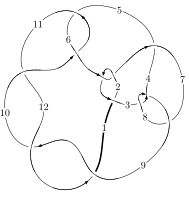
\includegraphics[width=112pt]{../../../GIT/diagram.site/Diagrams/png/2426_12n_0337.png}\\
\ \ \ A knot diagram\footnotemark}&
\allowdisplaybreaks
\textbf{Linearized knot diagam} \\
\cline{2-2}
 &
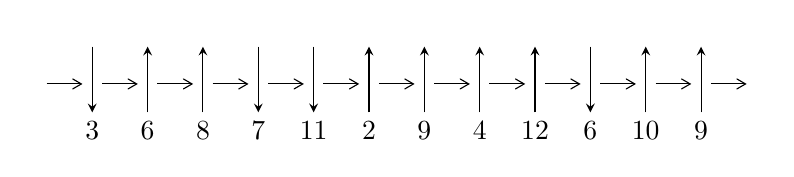
\begin{tikzpicture}[x=20pt, y=17pt]
	% nodes
	\node (C0) at (0, 0) {};
	\node (C1) at (1, 0) {};
	\node (C1U) at (1, +1) {};
	\node (C1D) at (1, -1) {3};

	\node (C2) at (2, 0) {};
	\node (C2U) at (2, +1) {};
	\node (C2D) at (2, -1) {6};

	\node (C3) at (3, 0) {};
	\node (C3U) at (3, +1) {};
	\node (C3D) at (3, -1) {8};

	\node (C4) at (4, 0) {};
	\node (C4U) at (4, +1) {};
	\node (C4D) at (4, -1) {7};

	\node (C5) at (5, 0) {};
	\node (C5U) at (5, +1) {};
	\node (C5D) at (5, -1) {11};

	\node (C6) at (6, 0) {};
	\node (C6U) at (6, +1) {};
	\node (C6D) at (6, -1) {2};

	\node (C7) at (7, 0) {};
	\node (C7U) at (7, +1) {};
	\node (C7D) at (7, -1) {9};

	\node (C8) at (8, 0) {};
	\node (C8U) at (8, +1) {};
	\node (C8D) at (8, -1) {4};

	\node (C9) at (9, 0) {};
	\node (C9U) at (9, +1) {};
	\node (C9D) at (9, -1) {12};

	\node (C10) at (10, 0) {};
	\node (C10U) at (10, +1) {};
	\node (C10D) at (10, -1) {6};

	\node (C11) at (11, 0) {};
	\node (C11U) at (11, +1) {};
	\node (C11D) at (11, -1) {10};

	\node (C12) at (12, 0) {};
	\node (C12U) at (12, +1) {};
	\node (C12D) at (12, -1) {9};
	\node (C13) at (13, 0) {};

	% arrows
	\draw[->,>={angle 60}]
	(C0) edge (C1) (C1) edge (C2) (C2) edge (C3) (C3) edge (C4) (C4) edge (C5) (C5) edge (C6) (C6) edge (C7) (C7) edge (C8) (C8) edge (C9) (C9) edge (C10) (C10) edge (C11) (C11) edge (C12) (C12) edge (C13) ;	\draw[->,>=stealth]
	(C1U) edge (C1D) (C2D) edge (C2U) (C3D) edge (C3U) (C4U) edge (C4D) (C5U) edge (C5D) (C6D) edge (C6U) (C7D) edge (C7U) (C8D) edge (C8U) (C9D) edge (C9U) (C10U) edge (C10D) (C11D) edge (C11U) (C12D) edge (C12U) ;
	\end{tikzpicture} \\
\hhline{~~} \\& 
\textbf{Solving Sequence} \\ \cline{2-2} 
 &
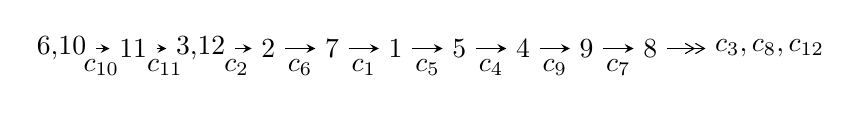
\begin{tikzpicture}[x=23pt, y=7pt]
	% node
	\node (A0) at (-1/8, 0) {6,10};
	\node (A1) at (1, 0) {11};
	\node (A2) at (33/16, 0) {3,12};
	\node (A3) at (25/8, 0) {2};
	\node (A4) at (33/8, 0) {7};
	\node (A5) at (41/8, 0) {1};
	\node (A6) at (49/8, 0) {5};
	\node (A7) at (57/8, 0) {4};
	\node (A8) at (65/8, 0) {9};
	\node (A9) at (73/8, 0) {8};
	\node (C1) at (1/2, -1) {$c_{10}$};
	\node (C2) at (3/2, -1) {$c_{11}$};
	\node (C3) at (21/8, -1) {$c_{2}$};
	\node (C4) at (29/8, -1) {$c_{6}$};
	\node (C5) at (37/8, -1) {$c_{1}$};
	\node (C6) at (45/8, -1) {$c_{5}$};
	\node (C7) at (53/8, -1) {$c_{4}$};
	\node (C8) at (61/8, -1) {$c_{9}$};
	\node (C9) at (69/8, -1) {$c_{7}$};
	\node (A10) at (11, 0) {$c_{3},c_{8},c_{12}$};

	% edge
	\draw[->,>=stealth]	
	(A0) edge (A1) (A1) edge (A2) (A2) edge (A3) (A3) edge (A4) (A4) edge (A5) (A5) edge (A6) (A6) edge (A7) (A7) edge (A8) (A8) edge (A9) ;
	\draw[->>,>={angle 60}]	
	(A9) edge (A10);
\end{tikzpicture} \\ 

\end{tabular} \\

\footnotetext{
The image of knot diagram is generated by the software ``\textbf{Draw programme}" developed by Andrew Bartholomew(\url{http://www.layer8.co.uk/maths/draw/index.htm\#Running-draw}), where we modified some parts for our purpose(\url{https://github.com/CATsTAILs/LinksPainter}).
}\phantom \\ \newline 
\centering \textbf{Ideals for irreducible components\footnotemark of $X_{\text{par}}$} 
 
\begin{align*}
I^u_{1}&=\langle 
8.75045\times10^{28} u^{62}+5.63839\times10^{29} u^{61}+\cdots+4.42036\times10^{29} b+4.19132\times10^{29},\\
\phantom{I^u_{1}}&\phantom{= \langle  }-8.61586\times10^{29} u^{62}+6.95817\times10^{29} u^{61}+\cdots+2.21018\times10^{29} a+3.02574\times10^{30},\;u^{63}- u^{62}+\cdots-10 u+1\rangle \\
I^u_{2}&=\langle 
u^5 b+u^3 b+2 u^2 b+b^2+2 b u- u^2- u-2,\;- u^4+a-1,\;u^6+u^4+2 u^2+1\rangle \\
\\
\end{align*}
\raggedright * 2 irreducible components of $\dim_{\mathbb{C}}=0$, with total 75 representations.\\
\footnotetext{All coefficients of polynomials are rational numbers. But the coefficients are sometimes approximated in decimal forms when there is not enough margin.}
\newpage
\renewcommand{\arraystretch}{1}
\centering \section*{I. $I^u_{1}= \langle 8.75\times10^{28} u^{62}+5.64\times10^{29} u^{61}+\cdots+4.42\times10^{29} b+4.19\times10^{29},\;-8.62\times10^{29} u^{62}+6.96\times10^{29} u^{61}+\cdots+2.21\times10^{29} a+3.03\times10^{30},\;u^{63}- u^{62}+\cdots-10 u+1 \rangle$}
\flushleft \textbf{(i) Arc colorings}\\
\begin{tabular}{m{7pt} m{180pt} m{7pt} m{180pt} }
\flushright $a_{6}=$&$\begin{pmatrix}0\\u\end{pmatrix}$ \\
\flushright $a_{10}=$&$\begin{pmatrix}1\\0\end{pmatrix}$ \\
\flushright $a_{11}=$&$\begin{pmatrix}1\\u^2\end{pmatrix}$ \\
\flushright $a_{3}=$&$\begin{pmatrix}3.89826 u^{62}-3.14824 u^{61}+\cdots+86.3365 u-13.6900\\-0.197958 u^{62}-1.27555 u^{61}+\cdots+12.6503 u-0.948184\end{pmatrix}$ \\
\flushright $a_{12}=$&$\begin{pmatrix}u^2+1\\u^2\end{pmatrix}$ \\
\flushright $a_{2}=$&$\begin{pmatrix}3.89826 u^{62}-3.14824 u^{61}+\cdots+86.3365 u-13.6900\\-0.929682 u^{62}-1.65830 u^{61}+\cdots+16.2523 u-1.69821\end{pmatrix}$ \\
\flushright $a_{7}=$&$\begin{pmatrix}1.53828 u^{62}-0.187645 u^{61}+\cdots+14.1508 u-6.97201\\2.72772 u^{62}-1.67622 u^{61}+\cdots+30.4294 u-4.29057\end{pmatrix}$ \\
\flushright $a_{1}=$&$\begin{pmatrix}u^6+u^4+2 u^2+1\\u^6+u^2\end{pmatrix}$ \\
\flushright $a_{5}=$&$\begin{pmatrix}u\\u^3+u\end{pmatrix}$ \\
\flushright $a_{4}=$&$\begin{pmatrix}0.471410 u^{62}-0.471626 u^{61}+\cdots+16.3283 u+1.49775\\-2.28058 u^{62}-0.384216 u^{61}+\cdots-9.13957 u+2.00704\end{pmatrix}$ \\
\flushright $a_{9}=$&$\begin{pmatrix}u^4+u^2+1\\u^4\end{pmatrix}$ \\
\flushright $a_{8}=$&$\begin{pmatrix}1.43450 u^{62}-0.861770 u^{61}+\cdots+27.0832 u-9.69122\\1.91211 u^{62}-0.548333 u^{61}+\cdots+17.6204 u-2.91399\end{pmatrix}$\\&\end{tabular}
\flushleft \textbf{(ii) Obstruction class $= -1$}\\~\\
\flushleft \textbf{(iii) Cusp Shapes $= 2.06158 u^{62}-4.22142 u^{61}+\cdots+98.6123 u-19.1903$}\\~\\
\newpage\renewcommand{\arraystretch}{1}
\flushleft \textbf{(iv) u-Polynomials at the component}\newline \\
\begin{tabular}{m{50pt}|m{274pt}}
Crossings & \hspace{64pt}u-Polynomials at each crossing \\
\hline $$\begin{aligned}c_{1}\end{aligned}$$&$\begin{aligned}
&u^{63}+23 u^{62}+\cdots-11050 u-625
\end{aligned}$\\
\hline $$\begin{aligned}c_{2},c_{6}\end{aligned}$$&$\begin{aligned}
&u^{63}- u^{62}+\cdots+40 u-25
\end{aligned}$\\
\hline $$\begin{aligned}c_{3},c_{8}\end{aligned}$$&$\begin{aligned}
&u^{63}- u^{62}+\cdots+2 u^2-1
\end{aligned}$\\
\hline $$\begin{aligned}c_{4}\end{aligned}$$&$\begin{aligned}
&u^{63}-3 u^{62}+\cdots+736 u-53
\end{aligned}$\\
\hline $$\begin{aligned}c_{5},c_{10}\end{aligned}$$&$\begin{aligned}
&u^{63}+u^{62}+\cdots-10 u-1
\end{aligned}$\\
\hline $$\begin{aligned}c_{7}\end{aligned}$$&$\begin{aligned}
&u^{63}-35 u^{62}+\cdots+4 u-1
\end{aligned}$\\
\hline $$\begin{aligned}c_{9},c_{11},c_{12}\end{aligned}$$&$\begin{aligned}
&u^{63}-23 u^{62}+\cdots+38 u+1
\end{aligned}$\\
\hline
\end{tabular}\\~\\
\newpage\renewcommand{\arraystretch}{1}
\flushleft \textbf{(v) Riley Polynomials at the component}\newline \\
\begin{tabular}{m{50pt}|m{274pt}}
Crossings & \hspace{64pt}Riley Polynomials at each crossing \\
\hline $$\begin{aligned}c_{1}\end{aligned}$$&$\begin{aligned}
&y^{63}+47 y^{62}+\cdots-20571250 y-390625
\end{aligned}$\\
\hline $$\begin{aligned}c_{2},c_{6}\end{aligned}$$&$\begin{aligned}
&y^{63}+23 y^{62}+\cdots-11050 y-625
\end{aligned}$\\
\hline $$\begin{aligned}c_{3},c_{8}\end{aligned}$$&$\begin{aligned}
&y^{63}-35 y^{62}+\cdots+4 y-1
\end{aligned}$\\
\hline $$\begin{aligned}c_{4}\end{aligned}$$&$\begin{aligned}
&y^{63}+49 y^{62}+\cdots+209280 y-2809
\end{aligned}$\\
\hline $$\begin{aligned}c_{5},c_{10}\end{aligned}$$&$\begin{aligned}
&y^{63}+23 y^{62}+\cdots+38 y-1
\end{aligned}$\\
\hline $$\begin{aligned}c_{7}\end{aligned}$$&$\begin{aligned}
&y^{63}-7 y^{62}+\cdots+4 y-1
\end{aligned}$\\
\hline $$\begin{aligned}c_{9},c_{11},c_{12}\end{aligned}$$&$\begin{aligned}
&y^{63}+39 y^{62}+\cdots+682 y-1
\end{aligned}$\\
\hline
\end{tabular}\\~\\
\newpage\flushleft \textbf{(vi) Complex Volumes and Cusp Shapes}
$$\begin{array}{c|c|c}  
\text{Solutions to }I^u_{1}& \I (\text{vol} + \sqrt{-1}CS) & \text{Cusp shape}\\
 \hline 
\begin{aligned}
u &= \phantom{-}0.615481 + 0.782024 I \\
a &= \phantom{-}0.924724 + 0.192341 I \\
b &= -0.085512 - 1.194750 I\end{aligned}
 & -2.81026 - 3.12410 I & \phantom{-}1.80668 + 2.74088 I \\ \hline\begin{aligned}
u &= \phantom{-}0.615481 - 0.782024 I \\
a &= \phantom{-}0.924724 - 0.192341 I \\
b &= -0.085512 + 1.194750 I\end{aligned}
 & -2.81026 + 3.12410 I & \phantom{-}1.80668 - 2.74088 I \\ \hline\begin{aligned}
u &= -0.817617 + 0.593503 I \\
a &= \phantom{-}1.176330 - 0.407742 I \\
b &= -0.666725 - 0.147698 I\end{aligned}
 & -0.28869 - 4.27274 I & \phantom{-0.000000 -}0. + 2.20858 I \\ \hline\begin{aligned}
u &= -0.817617 - 0.593503 I \\
a &= \phantom{-}1.176330 + 0.407742 I \\
b &= -0.666725 + 0.147698 I\end{aligned}
 & -0.28869 + 4.27274 I & \phantom{-0.000000 } 0. - 2.20858 I \\ \hline\begin{aligned}
u &= -0.822477 + 0.507948 I \\
a &= -0.501572 - 1.068710 I \\
b &= \phantom{-}0.080964 - 0.498715 I\end{aligned}
 & \phantom{-}4.20996 - 3.12624 I & \phantom{-}4.99490 + 1.04203 I \\ \hline\begin{aligned}
u &= -0.822477 - 0.507948 I \\
a &= -0.501572 + 1.068710 I \\
b &= \phantom{-}0.080964 + 0.498715 I\end{aligned}
 & \phantom{-}4.20996 + 3.12624 I & \phantom{-}4.99490 - 1.04203 I \\ \hline\begin{aligned}
u &= -0.654440 + 0.706606 I \\
a &= \phantom{-}1.004440 - 0.278481 I \\
b &= -0.521492 + 0.799483 I\end{aligned}
 & -3.29416 - 2.07147 I & -0.14477 + 3.47358 I \\ \hline\begin{aligned}
u &= -0.654440 - 0.706606 I \\
a &= \phantom{-}1.004440 + 0.278481 I \\
b &= -0.521492 - 0.799483 I\end{aligned}
 & -3.29416 + 2.07147 I & -0.14477 - 3.47358 I \\ \hline\begin{aligned}
u &= \phantom{-}0.822755 + 0.498425 I \\
a &= \phantom{-}1.246610 + 0.349007 I \\
b &= -0.388160 + 0.165493 I\end{aligned}
 & \phantom{-}4.25689 + 0.43803 I & \phantom{-}5.01449 + 0.38960 I \\ \hline\begin{aligned}
u &= \phantom{-}0.822755 - 0.498425 I \\
a &= \phantom{-}1.246610 - 0.349007 I \\
b &= -0.388160 - 0.165493 I\end{aligned}
 & \phantom{-}4.25689 - 0.43803 I & \phantom{-}5.01449 - 0.38960 I\\
 \hline 
 \end{array}$$\newpage$$\begin{array}{c|c|c}  
\text{Solutions to }I^u_{1}& \I (\text{vol} + \sqrt{-1}CS) & \text{Cusp shape}\\
 \hline 
\begin{aligned}
u &= -0.358362 + 0.992150 I \\
a &= -0.074839 - 0.827034 I \\
b &= -0.15062 - 1.56941 I\end{aligned}
 & \phantom{-}4.17413 + 3.04921 I & \phantom{-}11.13137 - 4.86659 I \\ \hline\begin{aligned}
u &= -0.358362 - 0.992150 I \\
a &= -0.074839 + 0.827034 I \\
b &= -0.15062 + 1.56941 I\end{aligned}
 & \phantom{-}4.17413 - 3.04921 I & \phantom{-}11.13137 + 4.86659 I \\ \hline\begin{aligned}
u &= \phantom{-}0.581922 + 0.742342 I \\
a &= -0.988921 - 0.922896 I \\
b &= \phantom{-}0.40243 - 1.83245 I\end{aligned}
 & -2.47100 + 1.06449 I & \phantom{-}2.36761 - 0.85729 I \\ \hline\begin{aligned}
u &= \phantom{-}0.581922 - 0.742342 I \\
a &= -0.988921 + 0.922896 I \\
b &= \phantom{-}0.40243 + 1.83245 I\end{aligned}
 & -2.47100 - 1.06449 I & \phantom{-}2.36761 + 0.85729 I \\ \hline\begin{aligned}
u &= \phantom{-}0.867209 + 0.606173 I \\
a &= \phantom{-}1.202120 + 0.457899 I \\
b &= -0.693184 + 0.345225 I\end{aligned}
 & \phantom{-}2.65432 + 9.47231 I & \phantom{-}4.00000 - 5.30483 I \\ \hline\begin{aligned}
u &= \phantom{-}0.867209 - 0.606173 I \\
a &= \phantom{-}1.202120 - 0.457899 I \\
b &= -0.693184 - 0.345225 I\end{aligned}
 & \phantom{-}2.65432 - 9.47231 I & \phantom{-}4.00000 + 5.30483 I \\ \hline\begin{aligned}
u &= \phantom{-}0.142481 + 0.926913 I \\
a &= \phantom{-}1.282780 - 0.021406 I \\
b &= \phantom{-}0.772343 - 0.206200 I\end{aligned}
 & \phantom{-}0.767985 + 0.824168 I & \phantom{-}9.41506 + 0.65151 I \\ \hline\begin{aligned}
u &= \phantom{-}0.142481 - 0.926913 I \\
a &= \phantom{-}1.282780 + 0.021406 I \\
b &= \phantom{-}0.772343 + 0.206200 I\end{aligned}
 & \phantom{-}0.767985 - 0.824168 I & \phantom{-}9.41506 - 0.65151 I \\ \hline\begin{aligned}
u &= -0.700176 + 0.840660 I \\
a &= -0.765140 + 0.730947 I \\
b &= \phantom{-}0.23555 + 1.51474 I\end{aligned}
 & -4.60599 + 2.68345 I & \phantom{-0.000000 } 0 \\ \hline\begin{aligned}
u &= -0.700176 - 0.840660 I \\
a &= -0.765140 - 0.730947 I \\
b &= \phantom{-}0.23555 - 1.51474 I\end{aligned}
 & -4.60599 - 2.68345 I & \phantom{-0.000000 } 0\\
 \hline 
 \end{array}$$\newpage$$\begin{array}{c|c|c}  
\text{Solutions to }I^u_{1}& \I (\text{vol} + \sqrt{-1}CS) & \text{Cusp shape}\\
 \hline 
\begin{aligned}
u &= \phantom{-}0.628609 + 0.908068 I \\
a &= \phantom{-}0.219058 + 0.696182 I \\
b &= \phantom{-}1.37912 + 1.43255 I\end{aligned}
 & -2.41121 - 1.77391 I & \phantom{-0.000000 } 0 \\ \hline\begin{aligned}
u &= \phantom{-}0.628609 - 0.908068 I \\
a &= \phantom{-}0.219058 - 0.696182 I \\
b &= \phantom{-}1.37912 - 1.43255 I\end{aligned}
 & -2.41121 + 1.77391 I & \phantom{-0.000000 } 0 \\ \hline\begin{aligned}
u &= -0.026642 + 0.893006 I \\
a &= -0.482850 - 0.230070 I \\
b &= -1.76148 - 0.77429 I\end{aligned}
 & \phantom{-}0.96850 - 2.33689 I & \phantom{-}10.51063 + 3.88561 I \\ \hline\begin{aligned}
u &= -0.026642 - 0.893006 I \\
a &= -0.482850 + 0.230070 I \\
b &= -1.76148 + 0.77429 I\end{aligned}
 & \phantom{-}0.96850 + 2.33689 I & \phantom{-}10.51063 - 3.88561 I \\ \hline\begin{aligned}
u &= \phantom{-}0.603817 + 0.944430 I \\
a &= -1.014530 - 0.651522 I \\
b &= -0.14337 - 1.71884 I\end{aligned}
 & -1.81973 - 5.79600 I & \phantom{-0.000000 } 0 \\ \hline\begin{aligned}
u &= \phantom{-}0.603817 - 0.944430 I \\
a &= -1.014530 + 0.651522 I \\
b &= -0.14337 + 1.71884 I\end{aligned}
 & -1.81973 + 5.79600 I & \phantom{-0.000000 } 0 \\ \hline\begin{aligned}
u &= \phantom{-}0.052552 + 1.129890 I \\
a &= -0.775773 - 0.796782 I \\
b &= -1.07864 - 2.15641 I\end{aligned}
 & \phantom{-}5.89708 - 3.19125 I & \phantom{-0.000000 } 0 \\ \hline\begin{aligned}
u &= \phantom{-}0.052552 - 1.129890 I \\
a &= -0.775773 + 0.796782 I \\
b &= -1.07864 + 2.15641 I\end{aligned}
 & \phantom{-}5.89708 + 3.19125 I & \phantom{-0.000000 } 0 \\ \hline\begin{aligned}
u &= -0.767293 + 0.838686 I \\
a &= -0.536133 + 0.727624 I \\
b &= \phantom{-}0.38652 + 1.38050 I\end{aligned}
 & -4.75625 + 2.66334 I & \phantom{-0.000000 } 0 \\ \hline\begin{aligned}
u &= -0.767293 - 0.838686 I \\
a &= -0.536133 - 0.727624 I \\
b &= \phantom{-}0.38652 - 1.38050 I\end{aligned}
 & -4.75625 - 2.66334 I & \phantom{-0.000000 } 0\\
 \hline 
 \end{array}$$\newpage$$\begin{array}{c|c|c}  
\text{Solutions to }I^u_{1}& \I (\text{vol} + \sqrt{-1}CS) & \text{Cusp shape}\\
 \hline 
\begin{aligned}
u &= -0.791545 + 0.338366 I \\
a &= -0.47232 - 1.36375 I \\
b &= \phantom{-}0.146940 - 0.685183 I\end{aligned}
 & \phantom{-}4.21373 + 5.84305 I & \phantom{-}4.20006 - 5.43025 I \\ \hline\begin{aligned}
u &= -0.791545 - 0.338366 I \\
a &= -0.47232 + 1.36375 I \\
b &= \phantom{-}0.146940 + 0.685183 I\end{aligned}
 & \phantom{-}4.21373 - 5.84305 I & \phantom{-}4.20006 + 5.43025 I \\ \hline\begin{aligned}
u &= -0.641851 + 0.958734 I \\
a &= \phantom{-}0.290568 - 0.785458 I \\
b &= \phantom{-}1.28323 - 2.11096 I\end{aligned}
 & -2.52965 + 7.13795 I & \phantom{-0.000000 } 0 \\ \hline\begin{aligned}
u &= -0.641851 - 0.958734 I \\
a &= \phantom{-}0.290568 + 0.785458 I \\
b &= \phantom{-}1.28323 + 2.11096 I\end{aligned}
 & -2.52965 - 7.13795 I & \phantom{-0.000000 } 0 \\ \hline\begin{aligned}
u &= \phantom{-}0.706658 + 0.446411 I \\
a &= -0.295145 + 1.196460 I \\
b &= \phantom{-}0.201963 + 0.567576 I\end{aligned}
 & \phantom{-}0.70382 - 1.36878 I & \phantom{-}1.16247 + 2.76782 I \\ \hline\begin{aligned}
u &= \phantom{-}0.706658 - 0.446411 I \\
a &= -0.295145 - 1.196460 I \\
b &= \phantom{-}0.201963 - 0.567576 I\end{aligned}
 & \phantom{-}0.70382 + 1.36878 I & \phantom{-}1.16247 - 2.76782 I \\ \hline\begin{aligned}
u &= -0.096687 + 1.163890 I \\
a &= -0.845889 + 0.838885 I \\
b &= -1.03193 + 2.21147 I\end{aligned}
 & \phantom{-}9.39173 + 8.34057 I & \phantom{-0.000000 } 0 \\ \hline\begin{aligned}
u &= -0.096687 - 1.163890 I \\
a &= -0.845889 - 0.838885 I \\
b &= -1.03193 - 2.21147 I\end{aligned}
 & \phantom{-}9.39173 - 8.34057 I & \phantom{-0.000000 } 0 \\ \hline\begin{aligned}
u &= \phantom{-}0.003658 + 1.168730 I \\
a &= -0.699048 + 0.871689 I \\
b &= -0.99139 + 2.10096 I\end{aligned}
 & \phantom{-}10.19250 - 1.37204 I & \phantom{-0.000000 } 0 \\ \hline\begin{aligned}
u &= \phantom{-}0.003658 - 1.168730 I \\
a &= -0.699048 - 0.871689 I \\
b &= -0.99139 - 2.10096 I\end{aligned}
 & \phantom{-}10.19250 + 1.37204 I & \phantom{-0.000000 } 0\\
 \hline 
 \end{array}$$\newpage$$\begin{array}{c|c|c}  
\text{Solutions to }I^u_{1}& \I (\text{vol} + \sqrt{-1}CS) & \text{Cusp shape}\\
 \hline 
\begin{aligned}
u &= \phantom{-}0.796964 + 0.882251 I \\
a &= -0.538356 - 0.100627 I \\
b &= \phantom{-}0.233347 - 0.784599 I\end{aligned}
 & -3.04388 - 0.13688 I & \phantom{-0.000000 } 0 \\ \hline\begin{aligned}
u &= \phantom{-}0.796964 - 0.882251 I \\
a &= -0.538356 + 0.100627 I \\
b &= \phantom{-}0.233347 + 0.784599 I\end{aligned}
 & -3.04388 + 0.13688 I & \phantom{-0.000000 } 0 \\ \hline\begin{aligned}
u &= -0.752341 + 0.920918 I \\
a &= -0.786716 + 0.409689 I \\
b &= \phantom{-}0.013060 + 1.198020 I\end{aligned}
 & -4.50104 + 3.08347 I & \phantom{-0.000000 } 0 \\ \hline\begin{aligned}
u &= -0.752341 - 0.920918 I \\
a &= -0.786716 - 0.409689 I \\
b &= \phantom{-}0.013060 - 1.198020 I\end{aligned}
 & -4.50104 - 3.08347 I & \phantom{-0.000000 } 0 \\ \hline\begin{aligned}
u &= \phantom{-}0.804318 + 0.888939 I \\
a &= -0.159292 - 0.605167 I \\
b &= \phantom{-}0.615657 - 1.226000 I\end{aligned}
 & -3.02941 - 5.85741 I & \phantom{-0.000000 } 0 \\ \hline\begin{aligned}
u &= \phantom{-}0.804318 - 0.888939 I \\
a &= -0.159292 + 0.605167 I \\
b &= \phantom{-}0.615657 + 1.226000 I\end{aligned}
 & -3.02941 + 5.85741 I & \phantom{-0.000000 } 0 \\ \hline\begin{aligned}
u &= \phantom{-}0.617710 + 1.047470 I \\
a &= \phantom{-}0.859697 - 0.364923 I \\
b &= \phantom{-}0.97715 - 1.06171 I\end{aligned}
 & \phantom{-}2.35789 - 3.68565 I & \phantom{-0.000000 } 0 \\ \hline\begin{aligned}
u &= \phantom{-}0.617710 - 1.047470 I \\
a &= \phantom{-}0.859697 + 0.364923 I \\
b &= \phantom{-}0.97715 + 1.06171 I\end{aligned}
 & \phantom{-}2.35789 + 3.68565 I & \phantom{-0.000000 } 0 \\ \hline\begin{aligned}
u &= -0.567021 + 1.085240 I \\
a &= \phantom{-}0.986354 + 0.368127 I \\
b &= \phantom{-}1.018770 + 0.967931 I\end{aligned}
 & \phantom{-}6.42352 - 0.87285 I & \phantom{-0.000000 } 0 \\ \hline\begin{aligned}
u &= -0.567021 - 1.085240 I \\
a &= \phantom{-}0.986354 - 0.368127 I \\
b &= \phantom{-}1.018770 - 0.967931 I\end{aligned}
 & \phantom{-}6.42352 + 0.87285 I & \phantom{-0.000000 } 0\\
 \hline 
 \end{array}$$\newpage$$\begin{array}{c|c|c}  
\text{Solutions to }I^u_{1}& \I (\text{vol} + \sqrt{-1}CS) & \text{Cusp shape}\\
 \hline 
\begin{aligned}
u &= -0.688188 + 1.054390 I \\
a &= \phantom{-}0.386516 - 0.981629 I \\
b &= \phantom{-}0.54971 - 2.74649 I\end{aligned}
 & \phantom{-}1.09750 + 9.92639 I & \phantom{-0.000000 } 0 \\ \hline\begin{aligned}
u &= -0.688188 - 1.054390 I \\
a &= \phantom{-}0.386516 + 0.981629 I \\
b &= \phantom{-}0.54971 + 2.74649 I\end{aligned}
 & \phantom{-}1.09750 - 9.92639 I & \phantom{-0.000000 } 0 \\ \hline\begin{aligned}
u &= \phantom{-}0.650788 + 1.081400 I \\
a &= \phantom{-}0.309480 + 1.022320 I \\
b &= \phantom{-}0.43116 + 2.53815 I\end{aligned}
 & \phantom{-}5.99769 - 5.93570 I & \phantom{-0.000000 } 0 \\ \hline\begin{aligned}
u &= \phantom{-}0.650788 - 1.081400 I \\
a &= \phantom{-}0.309480 - 1.022320 I \\
b &= \phantom{-}0.43116 - 2.53815 I\end{aligned}
 & \phantom{-}5.99769 + 5.93570 I & \phantom{-0.000000 } 0 \\ \hline\begin{aligned}
u &= -0.655982 + 1.078790 I \\
a &= \phantom{-}0.836188 + 0.475018 I \\
b &= \phantom{-}1.03372 + 1.10446 I\end{aligned}
 & \phantom{-}5.91225 + 8.64566 I & \phantom{-0.000000 } 0 \\ \hline\begin{aligned}
u &= -0.655982 - 1.078790 I \\
a &= \phantom{-}0.836188 - 0.475018 I \\
b &= \phantom{-}1.03372 - 1.10446 I\end{aligned}
 & \phantom{-}5.91225 - 8.64566 I & \phantom{-0.000000 } 0 \\ \hline\begin{aligned}
u &= \phantom{-}0.314549 + 0.662120 I \\
a &= \phantom{-}0.218311 + 0.670532 I \\
b &= -0.011835 + 0.612906 I\end{aligned}
 & \phantom{-}0.267822 - 1.158260 I & \phantom{-}3.61517 + 5.66198 I \\ \hline\begin{aligned}
u &= \phantom{-}0.314549 - 0.662120 I \\
a &= \phantom{-}0.218311 - 0.670532 I \\
b &= -0.011835 - 0.612906 I\end{aligned}
 & \phantom{-}0.267822 + 1.158260 I & \phantom{-}3.61517 - 5.66198 I \\ \hline\begin{aligned}
u &= \phantom{-}0.710541 + 1.068660 I \\
a &= \phantom{-}0.425206 + 1.016740 I \\
b &= \phantom{-}0.42500 + 2.83258 I\end{aligned}
 & \phantom{-}4.0664 - 15.3392 I & \phantom{-0.000000 } 0 \\ \hline\begin{aligned}
u &= \phantom{-}0.710541 - 1.068660 I \\
a &= \phantom{-}0.425206 - 1.016740 I \\
b &= \phantom{-}0.42500 - 2.83258 I\end{aligned}
 & \phantom{-}4.0664 + 15.3392 I & \phantom{-0.000000 } 0\\
 \hline 
 \end{array}$$\newpage$$\begin{array}{c|c|c}  
\text{Solutions to }I^u_{1}& \I (\text{vol} + \sqrt{-1}CS) & \text{Cusp shape}\\
 \hline 
\begin{aligned}
u &= -0.516415\phantom{ +0.000000I} \\
a &= \phantom{-}1.18250\phantom{ +0.000000I} \\
b &= -0.0216347\phantom{ +0.000000I}\end{aligned}
 & \phantom{-}1.52695\phantom{ +0.000000I} & \phantom{-}6.20940\phantom{ +0.000000I} \\ \hline\begin{aligned}
u &= \phantom{-}0.178816 + 0.052588 I \\
a &= \phantom{-}0.97689 + 5.20866 I \\
b &= \phantom{-}0.848518 + 0.314174 I\end{aligned}
 & -1.74489 - 2.05954 I & -4.07565 + 4.15680 I \\ \hline\begin{aligned}
u &= \phantom{-}0.178816 - 0.052588 I \\
a &= \phantom{-}0.97689 - 5.20866 I \\
b &= \phantom{-}0.848518 - 0.314174 I\end{aligned}
 & -1.74489 + 2.05954 I & -4.07565 - 4.15680 I\\
 \hline 
 \end{array}$$\newpage\newpage\renewcommand{\arraystretch}{1}
\centering \section*{II. $I^u_{2}= \langle u^5 b+u^3 b+2 u^2 b+b^2+2 b u- u^2- u-2,\;- u^4+a-1,\;u^6+u^4+2 u^2+1 \rangle$}
\flushleft \textbf{(i) Arc colorings}\\
\begin{tabular}{m{7pt} m{180pt} m{7pt} m{180pt} }
\flushright $a_{6}=$&$\begin{pmatrix}0\\u\end{pmatrix}$ \\
\flushright $a_{10}=$&$\begin{pmatrix}1\\0\end{pmatrix}$ \\
\flushright $a_{11}=$&$\begin{pmatrix}1\\u^2\end{pmatrix}$ \\
\flushright $a_{3}=$&$\begin{pmatrix}u^4+1\\b\end{pmatrix}$ \\
\flushright $a_{12}=$&$\begin{pmatrix}u^2+1\\u^2\end{pmatrix}$ \\
\flushright $a_{2}=$&$\begin{pmatrix}u^4+1\\- u^4- u^2+b-1\end{pmatrix}$ \\
\flushright $a_{7}=$&$\begin{pmatrix}u^5+u^3+2 u\\u^5 b+b u\end{pmatrix}$ \\
\flushright $a_{1}=$&$\begin{pmatrix}0\\- u^4- u^2-1\end{pmatrix}$ \\
\flushright $a_{5}=$&$\begin{pmatrix}u\\u^3+u\end{pmatrix}$ \\
\flushright $a_{4}=$&$\begin{pmatrix}u^5 b- u^5- u^3+b u\\- u^3 b+2 u^3+u^2+b+3 u\end{pmatrix}$ \\
\flushright $a_{9}=$&$\begin{pmatrix}u^4+u^2+1\\u^4\end{pmatrix}$ \\
\flushright $a_{8}=$&$\begin{pmatrix}u^5 b+u^5+u^3 b+b u+u\\2 u^5 b- u^5-2 u^3+b u- u\end{pmatrix}$\\&\end{tabular}
\flushleft \textbf{(ii) Obstruction class $= 1$}\\~\\
\flushleft \textbf{(iii) Cusp Shapes $= 4 u^4-4 u^3-4 b u+4 u^2+8$}\\~\\
\newpage\renewcommand{\arraystretch}{1}
\flushleft \textbf{(iv) u-Polynomials at the component}\newline \\
\begin{tabular}{m{50pt}|m{274pt}}
Crossings & \hspace{64pt}u-Polynomials at each crossing \\
\hline $$\begin{aligned}c_{1}\end{aligned}$$&$\begin{aligned}
&(u-1)^{12}
\end{aligned}$\\
\hline $$\begin{aligned}c_{2},c_{6}\end{aligned}$$&$\begin{aligned}
&(u^2+1)^6
\end{aligned}$\\
\hline $$\begin{aligned}c_{3},c_{4},c_{8}\end{aligned}$$&$\begin{aligned}
&(u^4- u^2+1)^3
\end{aligned}$\\
\hline $$\begin{aligned}c_{5},c_{10}\end{aligned}$$&$\begin{aligned}
&(u^6+u^4+2 u^2+1)^2
\end{aligned}$\\
\hline $$\begin{aligned}c_{7}\end{aligned}$$&$\begin{aligned}
&(u^2+u+1)^6
\end{aligned}$\\
\hline $$\begin{aligned}c_{9}\end{aligned}$$&$\begin{aligned}
&(u^3+u^2+2 u+1)^4
\end{aligned}$\\
\hline $$\begin{aligned}c_{11},c_{12}\end{aligned}$$&$\begin{aligned}
&(u^3- u^2+2 u-1)^4
\end{aligned}$\\
\hline
\end{tabular}\\~\\
\newpage\renewcommand{\arraystretch}{1}
\flushleft \textbf{(v) Riley Polynomials at the component}\newline \\
\begin{tabular}{m{50pt}|m{274pt}}
Crossings & \hspace{64pt}Riley Polynomials at each crossing \\
\hline $$\begin{aligned}c_{1}\end{aligned}$$&$\begin{aligned}
&(y-1)^{12}
\end{aligned}$\\
\hline $$\begin{aligned}c_{2},c_{6}\end{aligned}$$&$\begin{aligned}
&(y+1)^{12}
\end{aligned}$\\
\hline $$\begin{aligned}c_{3},c_{4},c_{8}\end{aligned}$$&$\begin{aligned}
&(y^2- y+1)^6
\end{aligned}$\\
\hline $$\begin{aligned}c_{5},c_{10}\end{aligned}$$&$\begin{aligned}
&(y^3+y^2+2 y+1)^4
\end{aligned}$\\
\hline $$\begin{aligned}c_{7}\end{aligned}$$&$\begin{aligned}
&(y^2+y+1)^6
\end{aligned}$\\
\hline $$\begin{aligned}c_{9},c_{11},c_{12}\end{aligned}$$&$\begin{aligned}
&(y^3+3 y^2+2 y-1)^4
\end{aligned}$\\
\hline
\end{tabular}\\~\\
\newpage\flushleft \textbf{(vi) Complex Volumes and Cusp Shapes}
$$\begin{array}{c|c|c}  
\text{Solutions to }I^u_{2}& \I (\text{vol} + \sqrt{-1}CS) & \text{Cusp shape}\\
 \hline 
\begin{aligned}
u &= \phantom{-}0.744862 + 0.877439 I \\
a &= -0.662359 - 0.562280 I \\
b &= \phantom{-}1.06984 - 1.15137 I\end{aligned}
 & -4.66906 - 0.79824 I & -1.50976 - 0.48465 I \\ \hline\begin{aligned}
u &= \phantom{-}0.744862 + 0.877439 I \\
a &= -0.662359 - 0.562280 I \\
b &= -0.07740 - 2.12527 I\end{aligned}
 & -4.66906 - 4.85801 I & -1.50976 + 6.44355 I \\ \hline\begin{aligned}
u &= \phantom{-}0.744862 - 0.877439 I \\
a &= -0.662359 + 0.562280 I \\
b &= \phantom{-}1.06984 + 1.15137 I\end{aligned}
 & -4.66906 + 0.79824 I & -1.50976 + 0.48465 I \\ \hline\begin{aligned}
u &= \phantom{-}0.744862 - 0.877439 I \\
a &= -0.662359 + 0.562280 I \\
b &= -0.07740 + 2.12527 I\end{aligned}
 & -4.66906 + 4.85801 I & -1.50976 - 6.44355 I \\ \hline\begin{aligned}
u &= -0.744862 + 0.877439 I \\
a &= -0.662359 + 0.562280 I \\
b &= \phantom{-}0.507560 + 0.489013 I\end{aligned}
 & -4.66906 + 4.85801 I & -1.50976 - 6.44355 I \\ \hline\begin{aligned}
u &= -0.744862 + 0.877439 I \\
a &= -0.662359 + 0.562280 I \\
b &= -0.63968 + 1.46291 I\end{aligned}
 & -4.66906 + 0.79824 I & -1.50976 + 0.48465 I \\ \hline\begin{aligned}
u &= -0.744862 - 0.877439 I \\
a &= -0.662359 - 0.562280 I \\
b &= \phantom{-}0.507560 - 0.489013 I\end{aligned}
 & -4.66906 - 4.85801 I & -1.50976 + 6.44355 I \\ \hline\begin{aligned}
u &= -0.744862 - 0.877439 I \\
a &= -0.662359 - 0.562280 I \\
b &= -0.63968 - 1.46291 I\end{aligned}
 & -4.66906 - 0.79824 I & -1.50976 - 0.48465 I \\ \hline\begin{aligned}
u &= \phantom{-0.000000 -}0.754878 I \\
a &= \phantom{-}1.32472\phantom{ +0.000000I} \\
b &= -0.577399 - 0.662359 I\end{aligned}
 & -0.53148 - 2.02988 I & \phantom{-}5.01951 + 3.46410 I \\ \hline\begin{aligned}
u &= \phantom{-0.000000 -}0.754878 I \\
a &= \phantom{-}1.32472\phantom{ +0.000000I} \\
b &= \phantom{-}1.71708 - 0.66236 I\end{aligned}
 & -0.53148 + 2.02988 I & \phantom{-}5.01951 - 3.46410 I\\
 \hline 
 \end{array}$$\newpage$$\begin{array}{c|c|c}  
\text{Solutions to }I^u_{2}& \I (\text{vol} + \sqrt{-1}CS) & \text{Cusp shape}\\
 \hline 
\begin{aligned}
u &= \phantom{-0.000000 } -0.754878 I \\
a &= \phantom{-}1.32472\phantom{ +0.000000I} \\
b &= -0.577399 + 0.662359 I\end{aligned}
 & -0.53148 + 2.02988 I & \phantom{-}5.01951 - 3.46410 I \\ \hline\begin{aligned}
u &= \phantom{-0.000000 } -0.754878 I \\
a &= \phantom{-}1.32472\phantom{ +0.000000I} \\
b &= \phantom{-}1.71708 + 0.66236 I\end{aligned}
 & -0.53148 - 2.02988 I & \phantom{-}5.01951 + 3.46410 I\\
 \hline 
 \end{array}$$\newpage
\newpage\renewcommand{\arraystretch}{1}
\centering \section*{ III. u-Polynomials}
\begin{tabular}{m{50pt}|m{274pt}}
Crossings & \hspace{64pt}u-Polynomials at each crossing \\
\hline $$\begin{aligned}c_{1}\end{aligned}$$&$\begin{aligned}
&((u-1)^{12})(u^{63}+23 u^{62}+\cdots-11050 u-625)
\end{aligned}$\\
\hline $$\begin{aligned}c_{2},c_{6}\end{aligned}$$&$\begin{aligned}
&((u^2+1)^6)(u^{63}- u^{62}+\cdots+40 u-25)
\end{aligned}$\\
\hline $$\begin{aligned}c_{3},c_{8}\end{aligned}$$&$\begin{aligned}
&((u^4- u^2+1)^3)(u^{63}- u^{62}+\cdots+2 u^2-1)
\end{aligned}$\\
\hline $$\begin{aligned}c_{4}\end{aligned}$$&$\begin{aligned}
&((u^4- u^2+1)^3)(u^{63}-3 u^{62}+\cdots+736 u-53)
\end{aligned}$\\
\hline $$\begin{aligned}c_{5},c_{10}\end{aligned}$$&$\begin{aligned}
&((u^6+u^4+2 u^2+1)^2)(u^{63}+u^{62}+\cdots-10 u-1)
\end{aligned}$\\
\hline $$\begin{aligned}c_{7}\end{aligned}$$&$\begin{aligned}
&((u^2+u+1)^6)(u^{63}-35 u^{62}+\cdots+4 u-1)
\end{aligned}$\\
\hline $$\begin{aligned}c_{9}\end{aligned}$$&$\begin{aligned}
&((u^3+u^2+2 u+1)^4)(u^{63}-23 u^{62}+\cdots+38 u+1)
\end{aligned}$\\
\hline $$\begin{aligned}c_{11},c_{12}\end{aligned}$$&$\begin{aligned}
&((u^3- u^2+2 u-1)^4)(u^{63}-23 u^{62}+\cdots+38 u+1)
\end{aligned}$\\
\hline
\end{tabular}\newpage\renewcommand{\arraystretch}{1}
\centering \section*{ IV. Riley Polynomials}
\begin{tabular}{m{50pt}|m{274pt}}
Crossings & \hspace{64pt}Riley Polynomials at each crossing \\
\hline $$\begin{aligned}c_{1}\end{aligned}$$&$\begin{aligned}
&((y-1)^{12})(y^{63}+47 y^{62}+\cdots-2.05713\times10^{7} y-390625)
\end{aligned}$\\
\hline $$\begin{aligned}c_{2},c_{6}\end{aligned}$$&$\begin{aligned}
&((y+1)^{12})(y^{63}+23 y^{62}+\cdots-11050 y-625)
\end{aligned}$\\
\hline $$\begin{aligned}c_{3},c_{8}\end{aligned}$$&$\begin{aligned}
&((y^2- y+1)^6)(y^{63}-35 y^{62}+\cdots+4 y-1)
\end{aligned}$\\
\hline $$\begin{aligned}c_{4}\end{aligned}$$&$\begin{aligned}
&((y^2- y+1)^6)(y^{63}+49 y^{62}+\cdots+209280 y-2809)
\end{aligned}$\\
\hline $$\begin{aligned}c_{5},c_{10}\end{aligned}$$&$\begin{aligned}
&((y^3+y^2+2 y+1)^4)(y^{63}+23 y^{62}+\cdots+38 y-1)
\end{aligned}$\\
\hline $$\begin{aligned}c_{7}\end{aligned}$$&$\begin{aligned}
&((y^2+y+1)^6)(y^{63}-7 y^{62}+\cdots+4 y-1)
\end{aligned}$\\
\hline $$\begin{aligned}c_{9},c_{11},c_{12}\end{aligned}$$&$\begin{aligned}
&((y^3+3 y^2+2 y-1)^4)(y^{63}+39 y^{62}+\cdots+682 y-1)
\end{aligned}$\\
\hline
\end{tabular}
\vskip 2pc
\end{document}